\chapter{動的に経路を選択して移動する機能の追加}
\label{chap:path_select}

\section{概要}
本章では,岡田らの従来手法に対して,目標とする進行方向のデータ
を加えることで,動的に経路を選択して移動する機能の追加を試みる.これにより,視覚に基づくナビゲーション
において,分岐路で「直進」「左折」などの任意の経路への移動
が可能となることを目指す.
以後,この動的に経路を選択して移動する機能を「経路選択機能」と呼ぶ
% \section{手法}
入力に目標方向を足した話
% \section{シミュレータを用いた実験}
シミュレータを用いて
経路選択機能の実験したよ.
% \section{実験結果}
同一の分岐路で,
選択できた

\section{経路選択機能を追加したシステム}
経路選択機能の追加を目的として,
データセットと学習器の入力へ,目標とする進行方向のデータ(以後,目標方向と呼ぶ)を新たに追加した.
\figref{fig:haru_mech_sys}に経路選択機能を追加したシステムを示す.
なお,上記の追加した要素を除き,他の部分は岡田らの従来手法と同様である.
学習時は,カメラ画像とメトリックマップに基づくルールベースの制御器から出力される
目標方向を入力としてデータセットへ加える.
岡田らの従来手法では,データセットの収集法に関して,いくつかバリエーションがある.
本論文では,その中で,最も経路追従の成功率が高い,学習器の出力とルールベース制御器の出力を比較し,
差の絶対値が閾値(0.05rad/s)を超えた場合のみ訓練データへ加える方法\cite{okada2021}を用いる.
学習後は,\figref{fig:path_select_abs}に示すように学習器へ外部から目標方向を入力する.
ロボットは視覚に基づくナビゲーションにおいて,入力された目標方向に従った経路を選択して移動する.

% 場所のデータのみ選択して訓練データに加える.
% 学習器の出力を監視して, 経路追従できない場所のデータのみ選択してデータセッ
% トに追加する手法を用いる.
\begin{figure}[htbp]
    \centering
     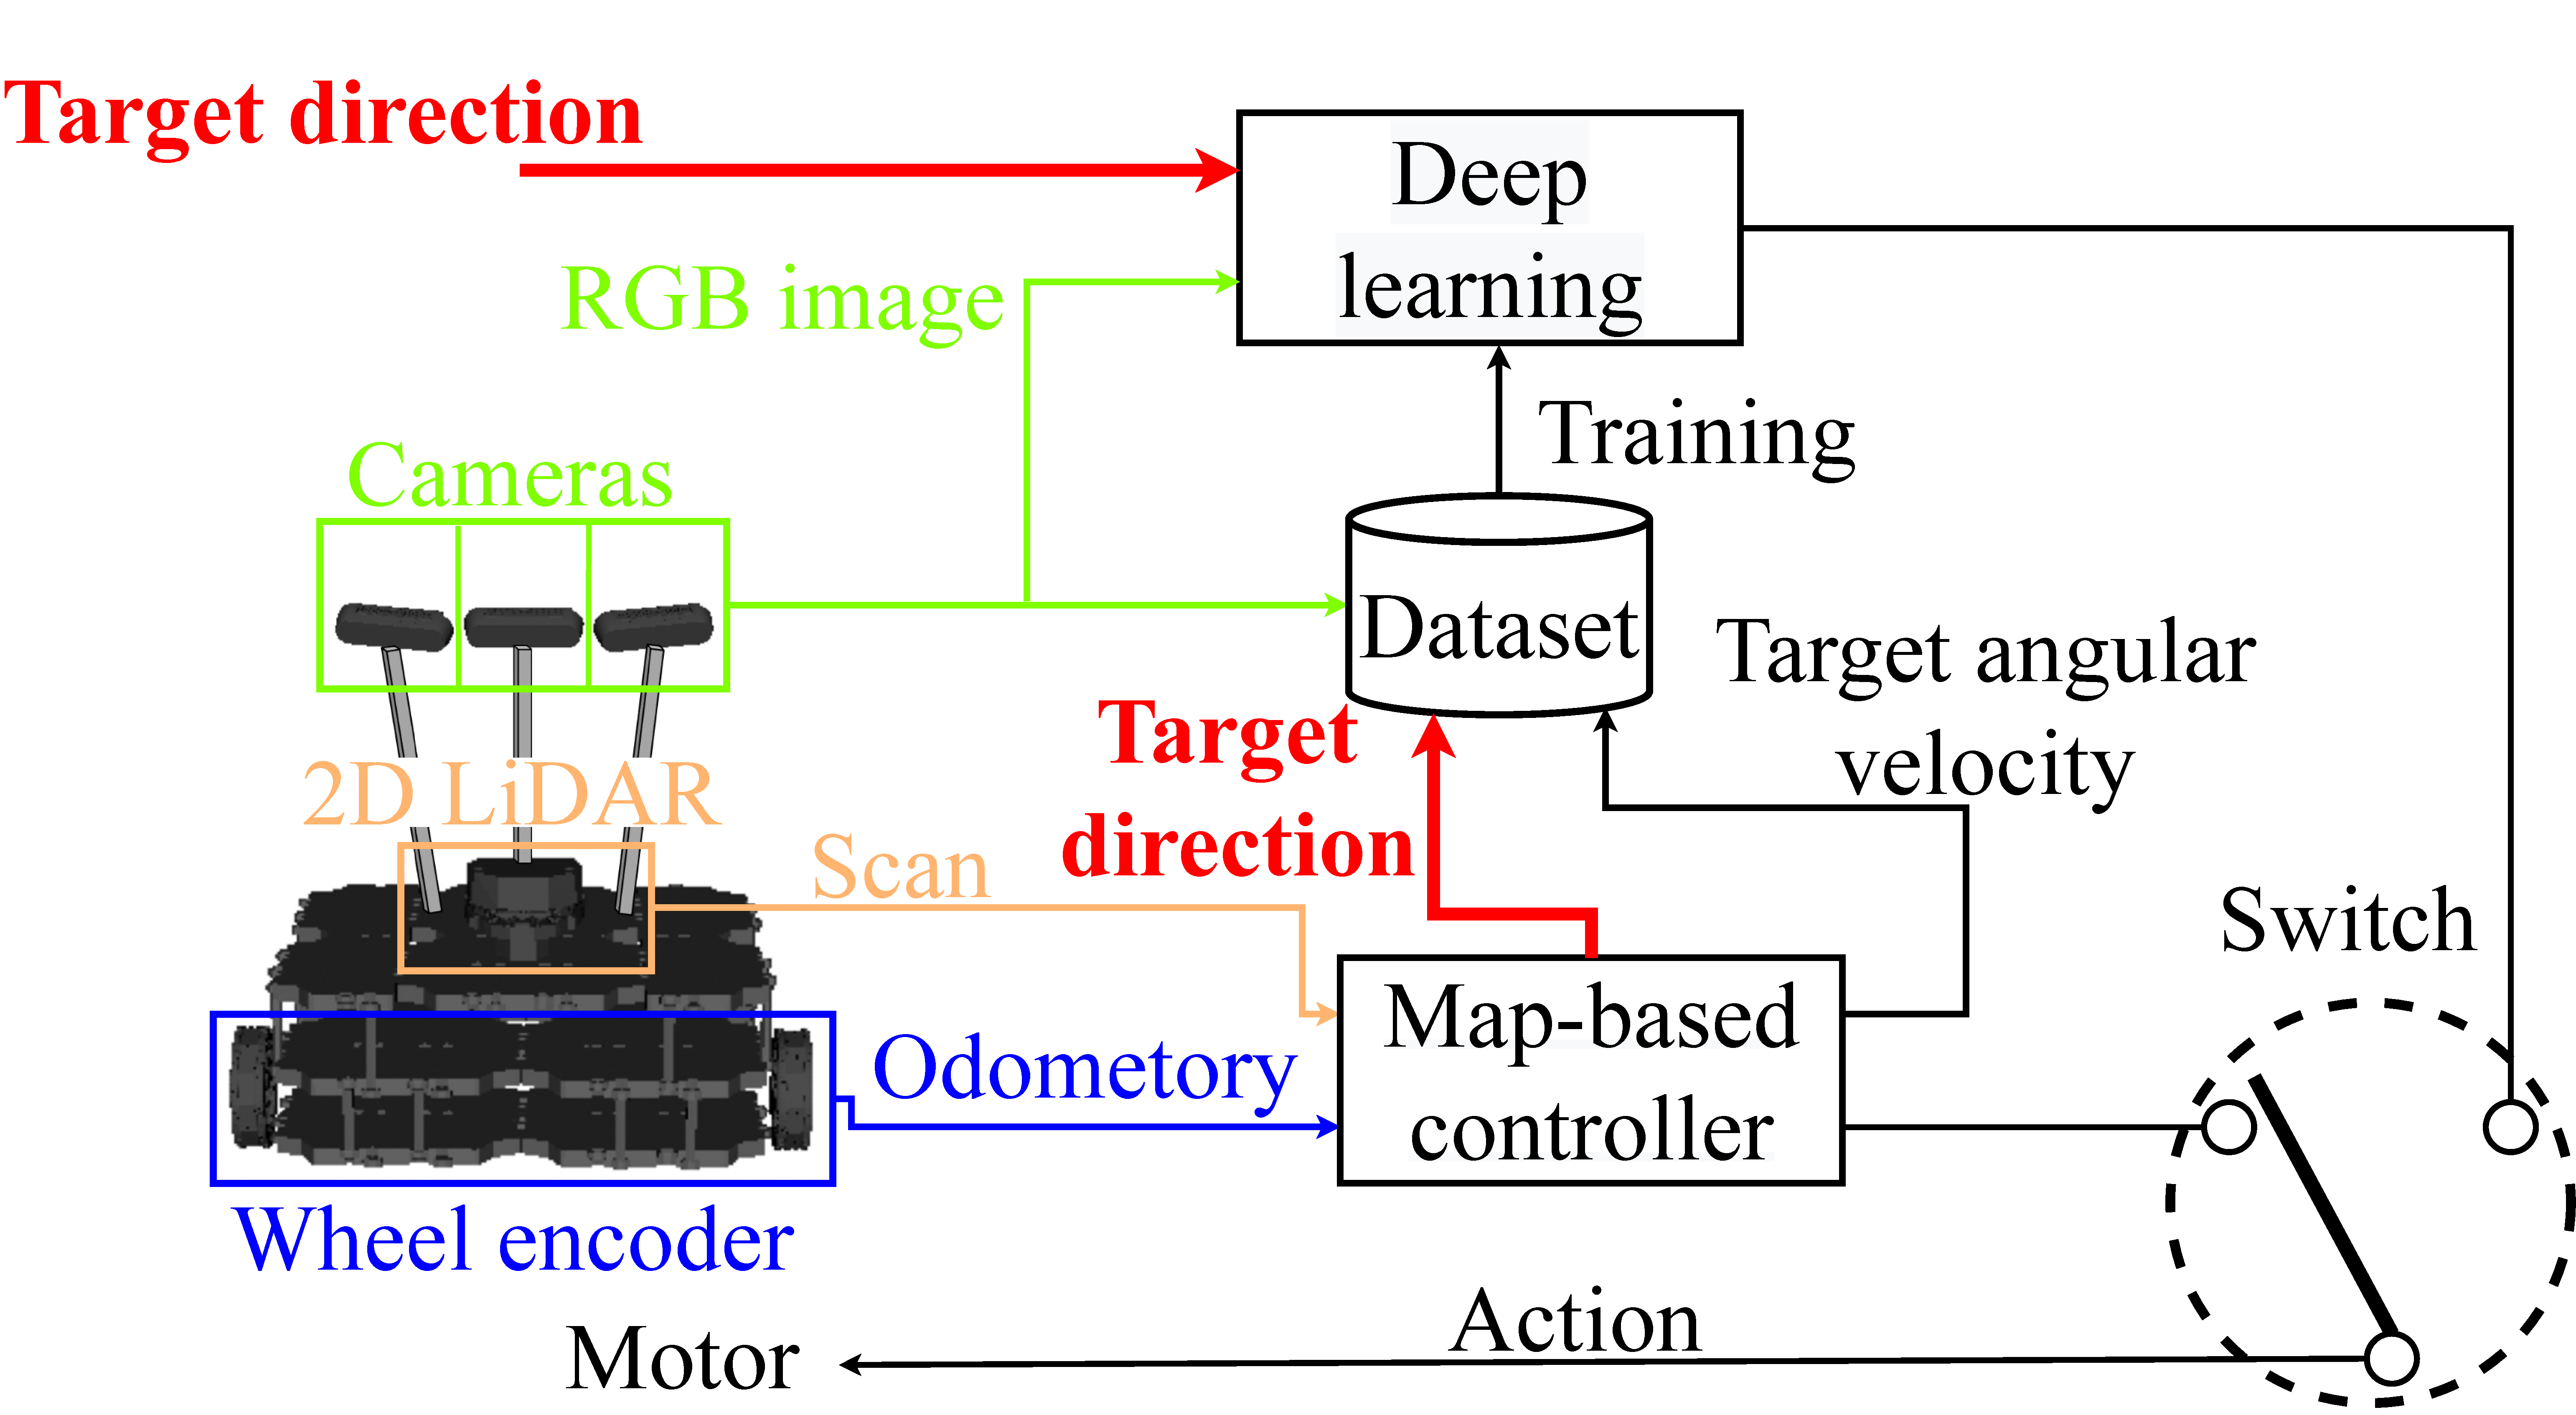
\includegraphics[width=130mm]{images/pdf/haru_mech_sys.pdf}
     \caption{System of the imitation learning with added function of
     selecting path}
     \label{fig:haru_mech_sys}
\end{figure}
\begin{figure}[htbp]
    \centering
     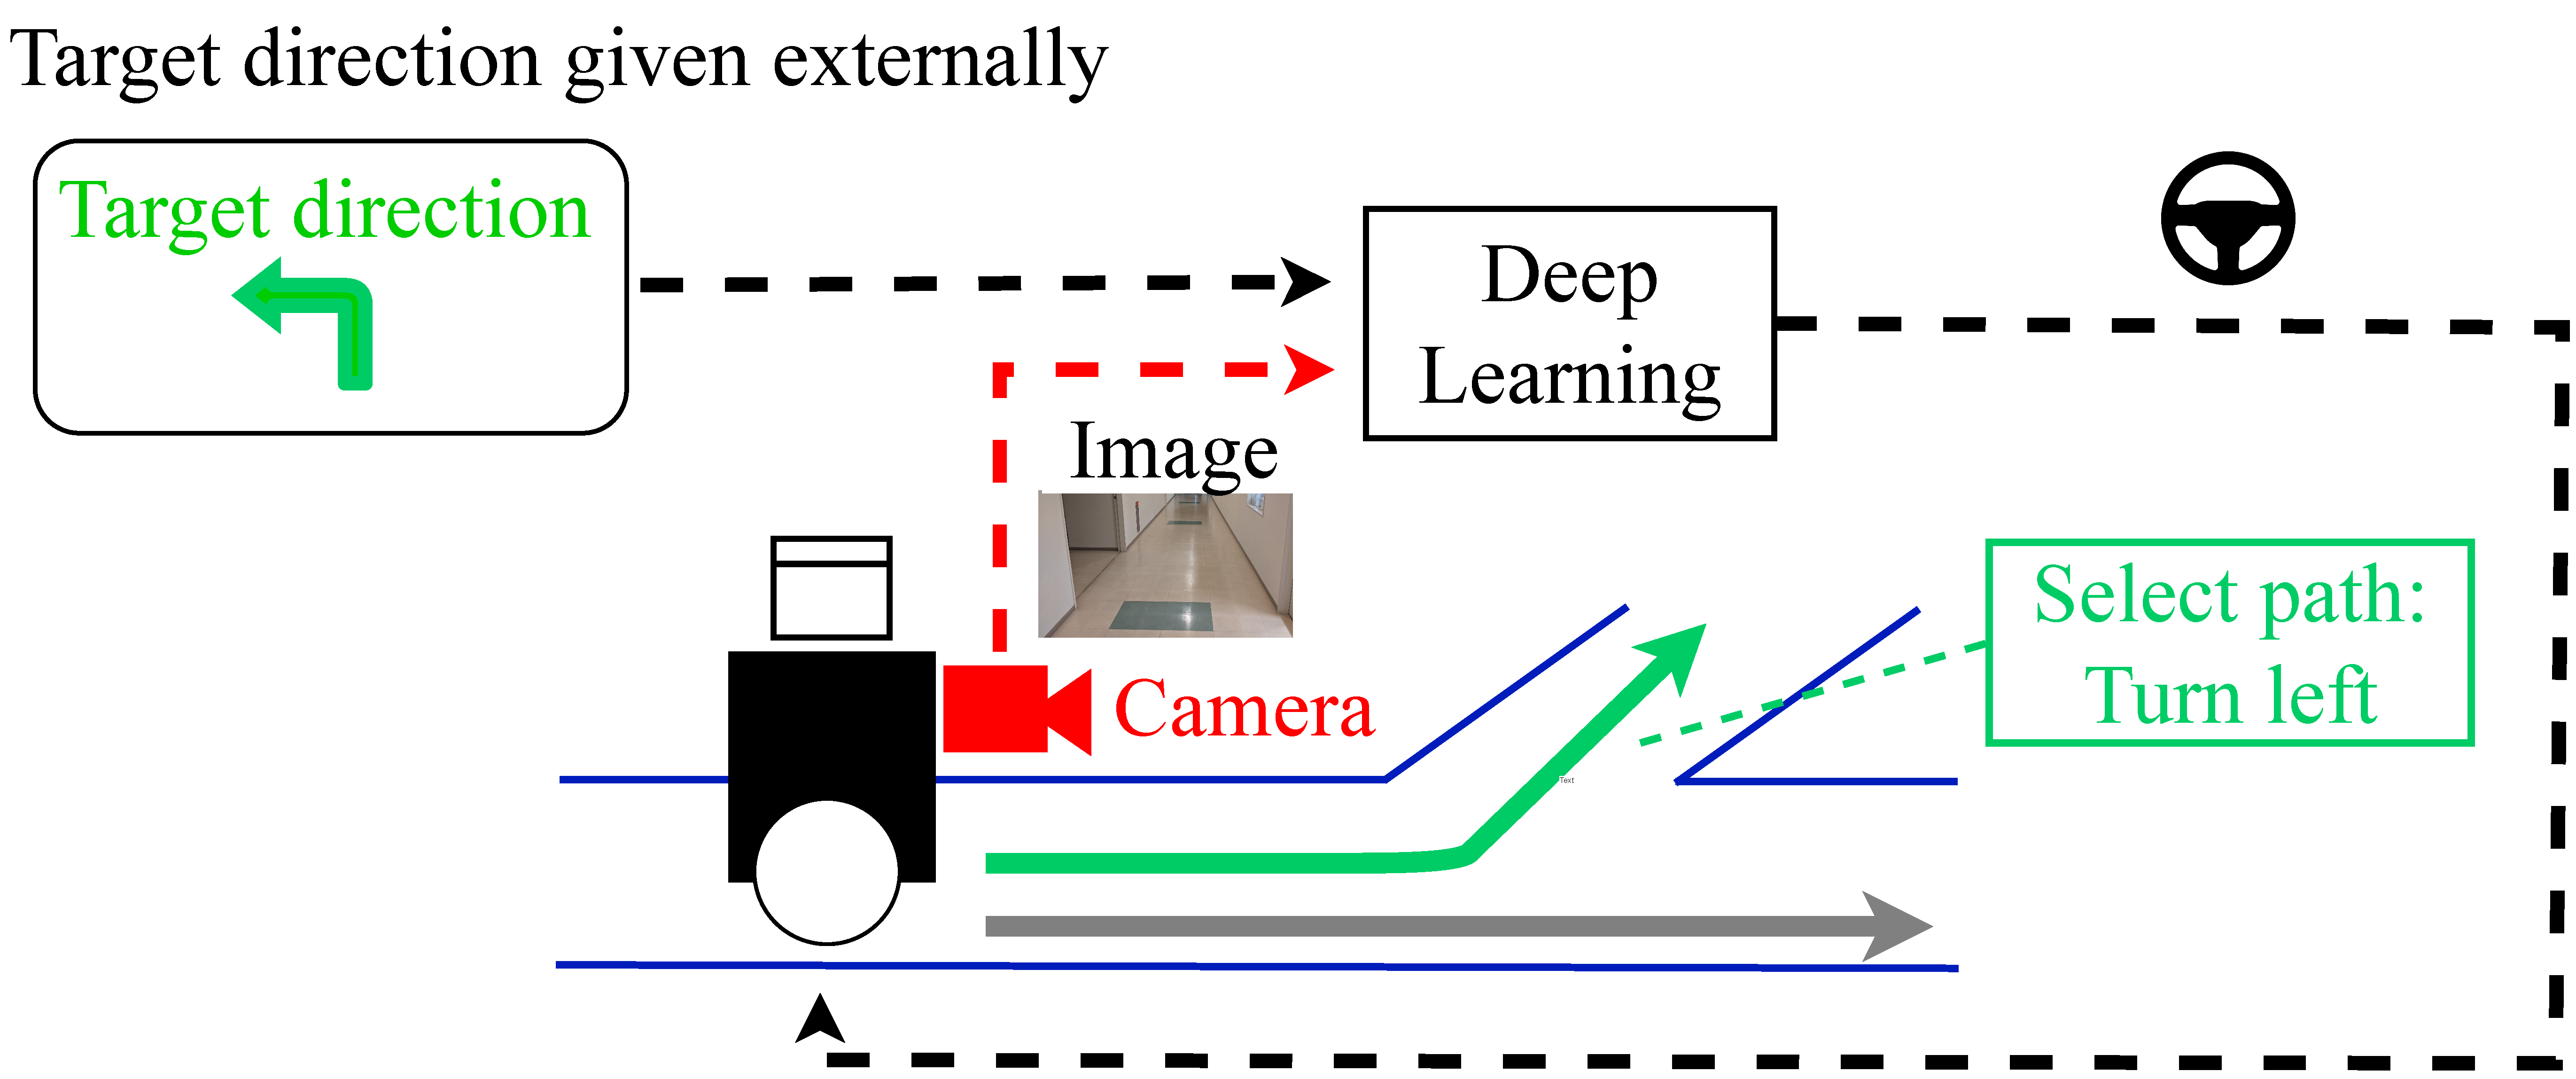
\includegraphics[width=130mm]{images/pdf/learning_gamma.pdf}
     \caption[Path selection and following behavior based on camera images 
     and target direction by imitation learning]{Path selection and following behavior based on camera images 
     and target direction by imitation learning(Quoted from \cite{haruyama2023})}
     \label{fig:path_select_abs}
\end{figure}

\clearpage
\subsubsection{ネットワークの構造と目標方向のデータ形式}
経路選択機能を追加した学習器のネットワークの構造を\figref{fig:haru_mech_net}に示す.
岡田らの従来手法で用いたネットワークの出力部に,目標方向の入力部を追加した.
この層に\tabref{tab:target_old}に示すワンホットベクトルの
データを入力する.
ネットワークは,画像を処理するCNNアーキテクチャ,
CNNの出力と目標方向を入力とする全結合層で構成されている.
損失関数や活性化関数などのパラメータは岡田らの従来手法と同様である.

学習器はRGB画像と,目標方向を入力,ヨー方向の角速度を出力として
end-to-end学習する.
つまり,視覚を入力とした行動を.目標方向によって条件付けながら学習する.
% 目標方向の
% 継続,直進,左折,右折の4つを
% ワンホットベクトルで表現する.
\begin{figure}[htbp]
    \centering
     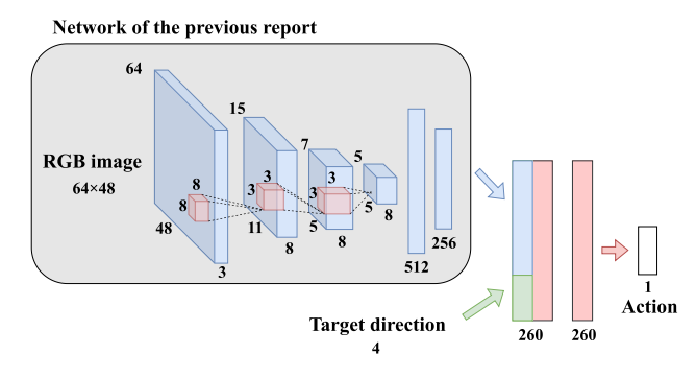
\includegraphics[width=130mm]{images/pdf/haru_mech.pdf}
     \caption[Structure of network with added function of
     selecting path]{Structure of network with added function of
     selecting path(Quoted from \cite{haruyama2023})}
     \label{fig:haru_mech_net}
\end{figure}

\begin{table}[htbp]
    \centering
    \caption{Target direction and data for imitation learning}\label{tab:target_old}
    \begin{tabular}{|c|c|}
    \hline
    Target direction & Data        \\
    \hline
    Continue   & {[}100,0,0,0{]} \\
    Go straight   & {[}0,100,0,0{]} \\
    Turn left   & {[}0,0,100,0{]} \\
    Turn right   & {[}0,0,0,100{]} \\
    \hline
    \end{tabular}
    \end{table}

\newpage
\section{シミュレータを用いた経路選択機能を確認する実験}
経路選択機能を追加したシステムで,指定した進行方向にロボットが移動できることを
シミュレータを用いた実験により確認する.
\subsubsection{実験装置}
実験はシミュレータ上で行い,シミュレータにはGazebo\cite{Gazebo}を使用し,
ロボットには\figref{fig:turtlebot3}に示すTurtleBot3 Waffle Pi\cite{ROBOTIS}へ3つのカメラを追加したモデルを用いる.
実験環境には,\figref{fig:haru_mech_exp}に示す千葉工業大学津田沼キャンパス2号館3階を模したモデルを用いた.
環境中のA,Bの地点においては,\figref{fig:haru_mech_exp_ab}に示すように侵入する方向が3つ,脱出する経路はそれぞれ2つ
あるため,バリエーションは6つある.
つまり,目標方向に従って適切に経路を選択して移動することが求められる場所となる
\begin{figure}[htbp]
    \centering
     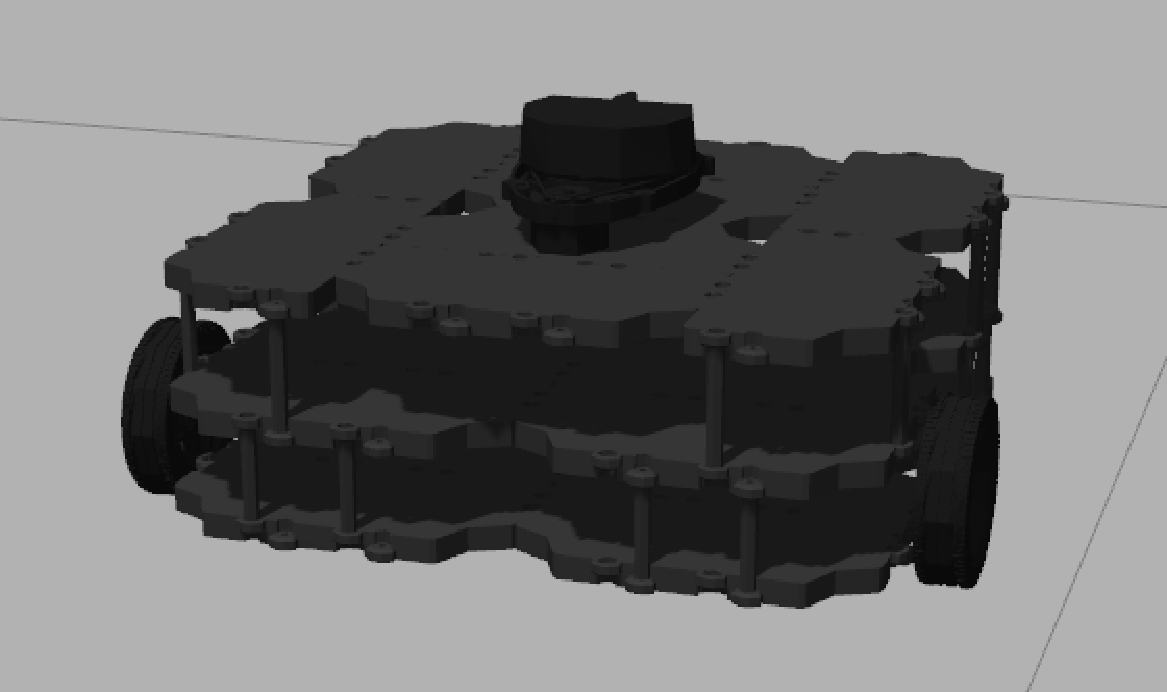
\includegraphics[width=80mm]{images/pdf/turtlebot3.pdf}
     \caption{TurtleBot3 Waffle Pi}
     \label{fig:turtlebot3}
\end{figure}
\begin{figure}[htbp]
    \centering
     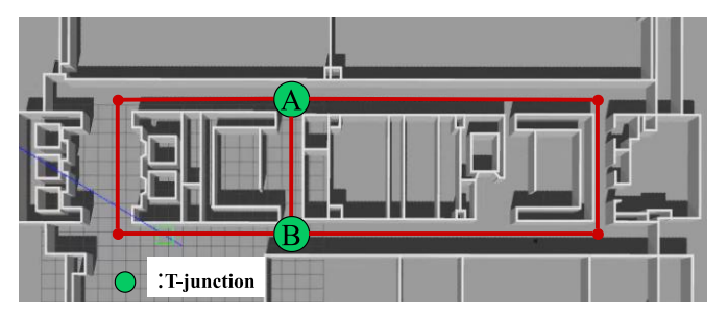
\includegraphics[width=130mm]{images/pdf/haru_mech_exp.pdf}
     \caption[Experimental environment of selecting path]{Experimental environment of selecting path(Quoted from \cite{haruyama2022})}
     \label{fig:haru_mech_exp}
\end{figure}
\begin{figure}[htbp]
    \centering
     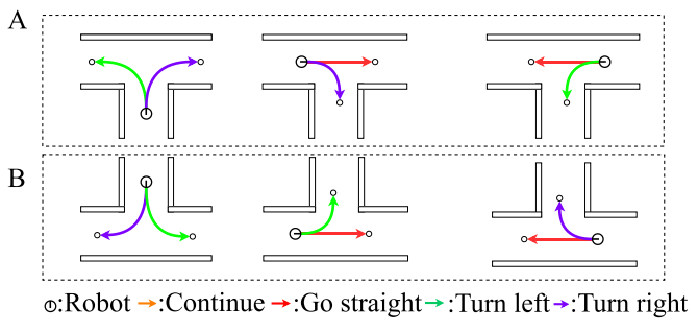
\includegraphics[width=130mm]{images/pdf/haru_mech_exp_ab.pdf}
     \caption[Selecting a path at the T-junction]{Selecting a path at the T-junction(Quoted from \cite{haruyama2022})}
     \label{fig:haru_mech_exp_ab}
\end{figure}
\vspace{-1zh}
\subsubsection{実験方法}
実験では,\figref{fig:haru_mech_route}に示した経路をaからfの順番で繰り返し走
行しながら,模倣学習を行う.目標方向のデータはメトリックマップに基づくルールベース制御器から出力
され,データセットに加えられる.学習は60000ステップ実行し,
その後視覚に基づくナビゲーションへ移行する.視覚に基づくナビゲーションにおいても
aからfまでの経路をロボットに走行させる.ロボットが壁に衝突した場合は,
ロボットを経路の中央まで戻して実験を継続する.
この実験を10回実施する.

\begin{figure}[htbp]
    \centering
     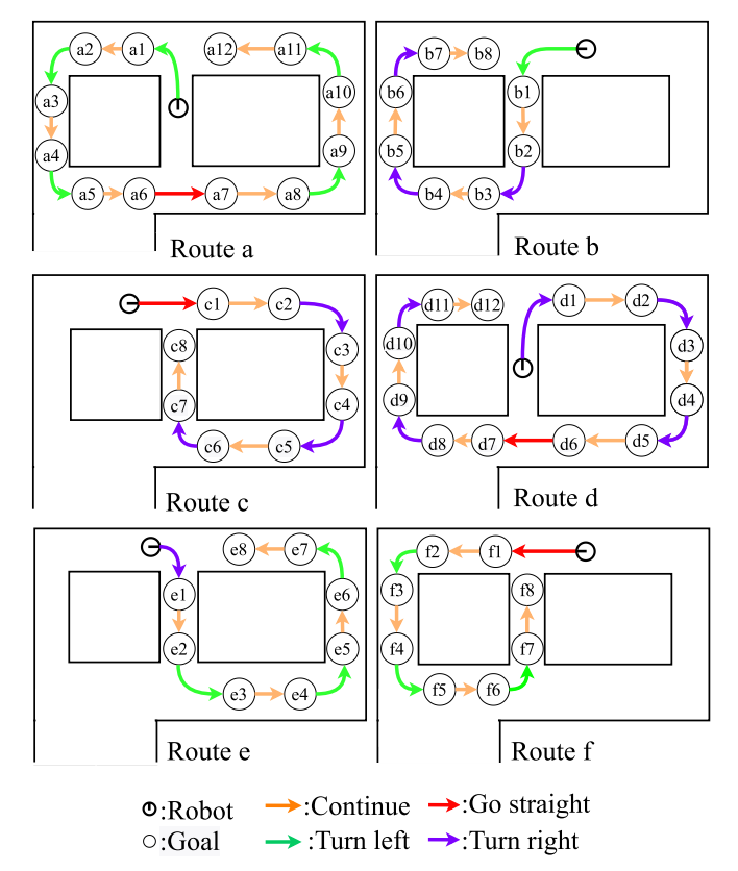
\includegraphics[width=130mm]{images/pdf/haru_mech_route.pdf}
     \caption[Route for experiment of selecting path]{Route for experiment of selecting path(Quoted from \cite{haruyama2022})}
     \label{fig:haru_mech_route}
\end{figure}
\clearpage
\subsubsection{実験結果}
実験結果を\figref{fig:haru_mech_ab_res}に示す.
図はA,Bそれぞれの分岐路で,ロボットが正しく経路を選択した回数を示している.
図に示すように,目標方向に従い113/120回適切に経路を選択する様子が
確認できた.ただし,\tabref{tab:path_res}に示した箇所では,壁に衝突するな
どして自律移動が継続できない様子も見られた.

\figref{fig:haru_mech_a_select}にA地
点で目標方向のコマンドに従い,ロボットが経路を選択して
走行する様子を示す.このように,同一の分岐路であっても目
標方向の入力に従い,ロボットが適切に経路を選択して走行
する様子が見られた.
この結果から,岡田らの従来手法に対し,任意の目的地に向けた移動に必要な,動的に経路を選択して移動する機能を
追加できたと考えられる,
% \vspace{5zh}
\begin{figure}[htbp]
    \centering
     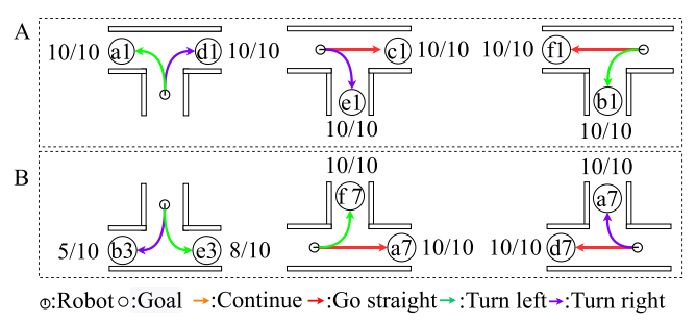
\includegraphics[width=130mm]{images/pdf/haru_mech_res.pdf}
     \caption[Number of times a correct path was selected]{Number of times a correct path was selected(Quoted from \cite{haruyama2022})}
     \label{fig:haru_mech_ab_res}
\end{figure}
\vspace{-1zh}
\begin{table}[htbp]
    \centering
    \caption{Location where the robot went off course}\label{tab:path_res}
    \begin{tabular}{|c|c|c|}
    \hline
    Location & Number of Failed        \\
    \hline
    a5   & 2/10 \\
    b3   & 5/10 \\
    d11   & 1/10 \\
    e1  &  2/10 \\
    f5    & 2/10 \\
    \hline
    \end{tabular}
    \end{table}
\begin{figure}[htbp]
    \centering
    %  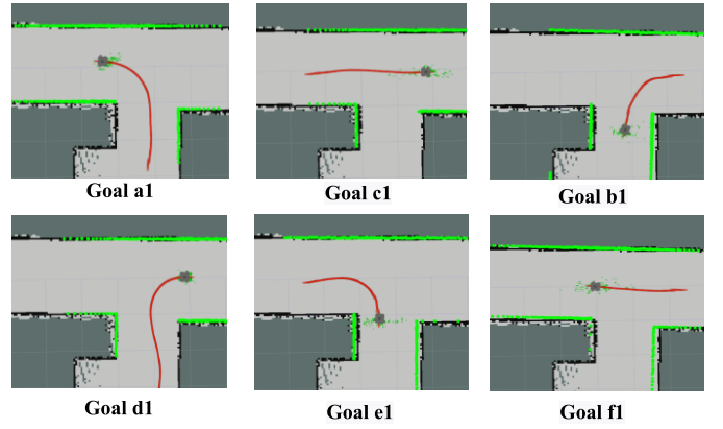
\includegraphics[width=120mm]{images/pdf/haru_mech_a_select.pdf}
     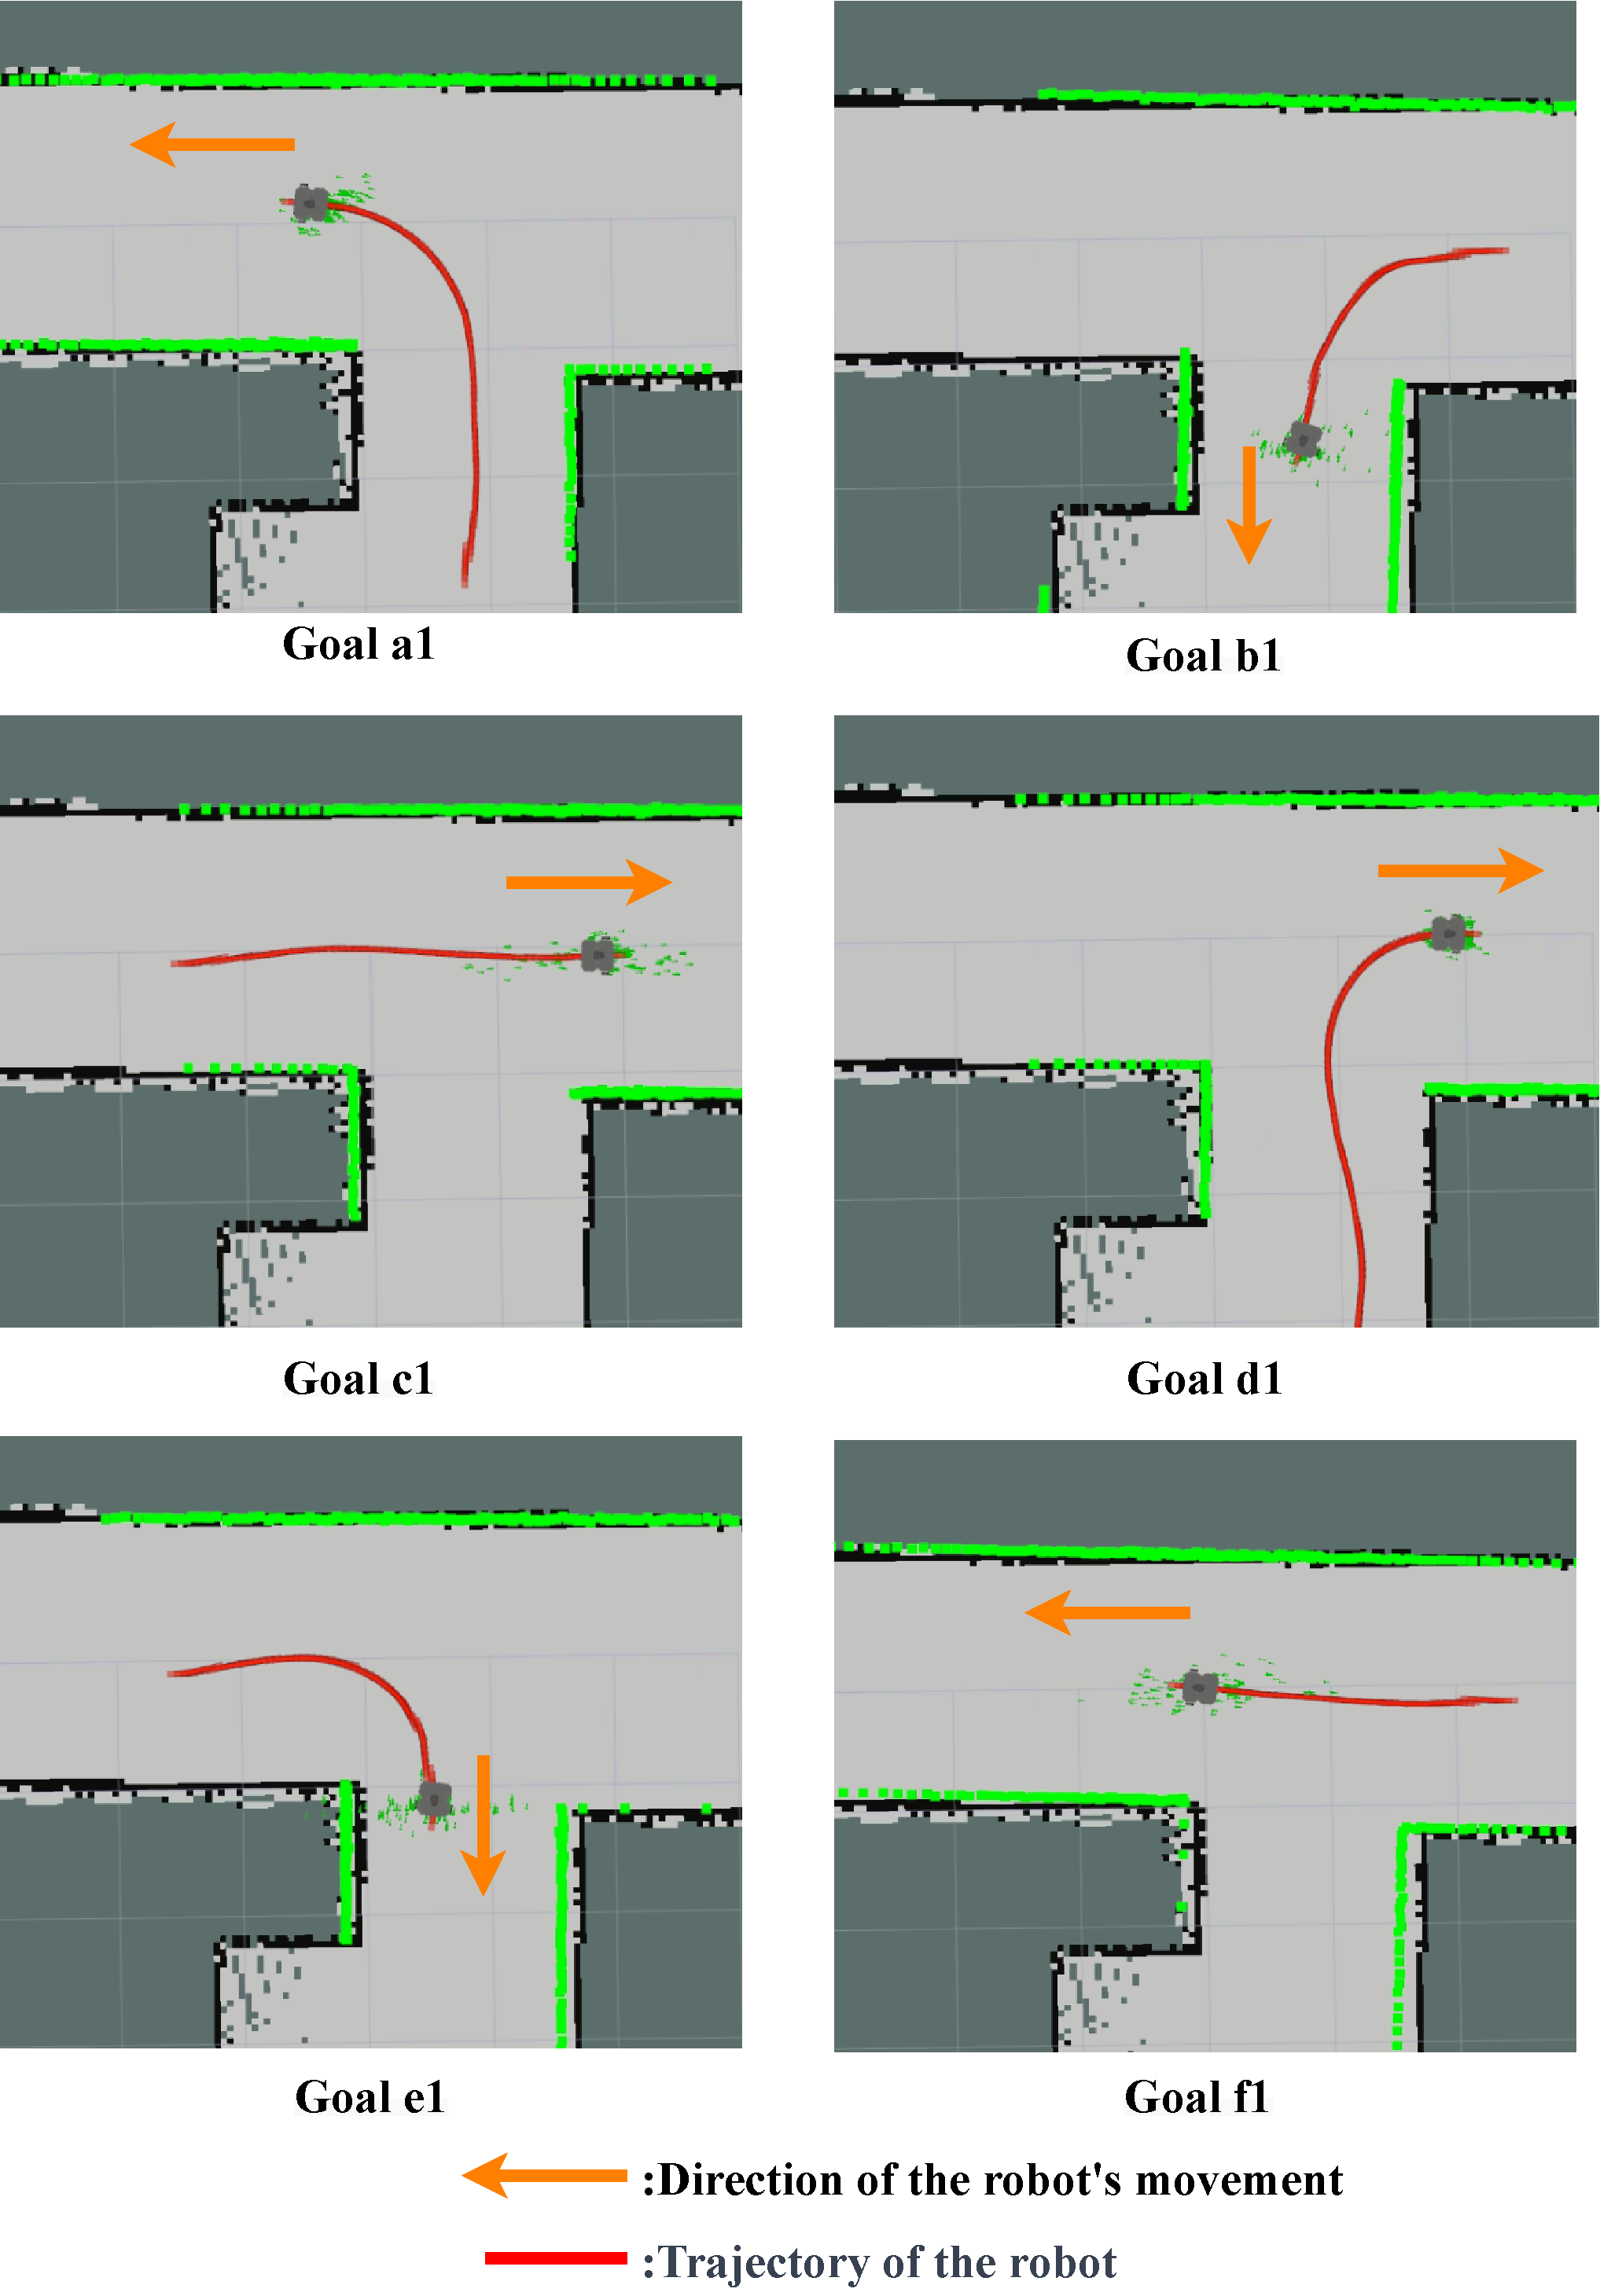
\includegraphics[width=130mm]{images/pdf/zyuziroute-select_a.pdf}
     \caption[The robot moving while selecting a path]{The robot moving while selecting a path(Quoted from \cite{haruyama2022})}
     \label{fig:haru_mech_a_select}
\end{figure}
